\documentclass[]{article}
\usepackage[utf8]{inputenc}
\usepackage[english]{babel}
\usepackage{graphicx}
\usepackage{hyperref}
\usepackage{appendix}
\hypersetup{
	colorlinks=true,
	linkcolor=blue,
	filecolor=magenta,      
	urlcolor=cyan,
}
\usepackage{mathtools}
\usepackage{float}   %this package is for placing graphs and tables in where the TeX is
\graphicspath{{images/}{../images/}}

\usepackage{blindtext}

\usepackage{subfiles}
\usepackage{verbatim}
\providecommand{\EqDir}{Equations}
\providecommand{\RefDir}{References}
\providecommand{\TableDir}{Tables}

\usepackage{apacite}
\usepackage{geometry}
\geometry{legalpaper, margin=1in}

\title{A Replication of Carroll(1997)\protect\footnote{A jupyter notebook replication of Carroll (1997) is available \href{https://github.com/sonjeongwon621/project-with-yusuf/blob/master/Carroll_1997_RemARK.ipynb}{here}}}
\author{Yusuf Suha Kulu, Jeongwon (John) Son, and Mingzuo Sun}
\date{}

\begin{document}
\setlength\parindent{0pt}
%\linespread{2}

\maketitle

\section{Summary}

This paper argues that the saving behaviour of a household is better described by the buffer stock version of the Life Cycle/Permanent Income Hypothesis (LC/PIH) than the traditional version of it. Buffer Stock Consumers set average consumption growth equal to average labor income growth, regardless of tastes. The buffer stock model predicts a higher marginal propensity to consume (MPC) out of transitory income, higher effective discount rate for future labor income, and a positive sign for the correlation between saving and expected labor income growth.\\

The finite horizon version of the model presented in the paper explains three emprical puzzles.
\begin{itemize}
\item \textbf{Consumption/income parallel:}Aggregate consumption parallels growth in income over periods of more than a few years.
\item \textbf{Consumption/income divergence:} For individual households, consumption is far from current income. This implies the consumption/income parallel does not arise at the household level.
\item \textbf{Stability of the household age/wealth profile:}The effects of the productivity growth slowdown after 1973 on the age/median-wealth profile and the extraordinarily high volatility of the household liquid wealth are explained. 
\end{itemize}

\newpage 

\section{Model Setup}

The consumer solves the following intertemporal optimization problem.\\
\begin{align}
\max \quad E_t \Sigma_{n=0}^{T-t} \beta^{n}u(c_{t+n})
\end{align}

\begin{align} \text{s.t.} \quad b_{t+1} &= R[b_t + y_t - c_t]\\
y_t &= p_tv_t\\
p_t &= G_tp_{t-1}n_t 
\end{align}

\bigskip

$y$: current labor income \\

$p$: permanent labor income \\

$v$: transitory income shock \\

$n$: permanent income shock \\

$G = (1+g)$: growth factor for permanent labor income \\

$b$: stock of physical net wealth \\

$R = (1+r)$: gross interest rate \\

$\beta = 1/(1+\delta)$: discount factor \\

Solving the consumer's optimization problem gives the following Euler equation.\\
\begin{align}
	1= R\beta E_{t-1}[\{c_t[R[m_{t-1}-c_{t-1}]/Gn_t + v_t]Gn_t/c_{t-1}\}^{-\rho}]
\end{align}

Lower case variables are defined as the uppercase variables divided by the current level of permanent income. \\

$m = b+y$: gross wealth \\

Since this is a life cycle model, the consumer consumes everything in the last period:$c_T[m_T] = m_T$. This implies that by recursion, the Euler equation gives the consumption ratio for each period. \\

If shocks to consumption are assumed to be lognormally distributed, a log-linearized version of the Euler equation takes the following form.\\
\begin{align}
	1= R\beta E_{t-1}[\{c_t[R[m_{t-1}-c_{t-1}]/Gn_t + v_t]Gn_t/c_{t-1}\}^{-\rho}]
\end{align}

\newpage

\section{Target wealth and consumption ratio}
There is a target of consumption ratio and wealth ratio for the infinite horizon buffer stock model. This can be seen in the figure below.\\

\begin{figure}[h]
\centerline{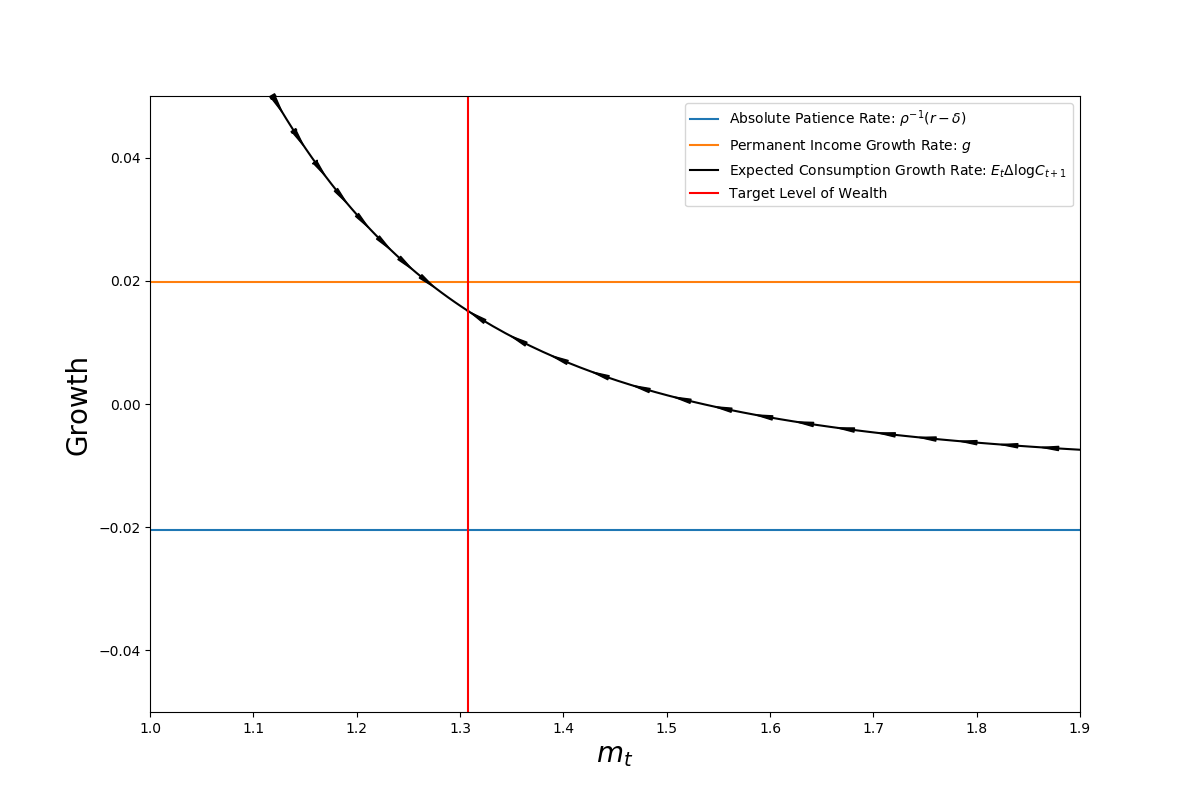
\includegraphics[width=6in]{Figures/Figure1a.png}}
\label{figure:1}
\caption{Expected Consumption Growth as a Function of Cash on Hand}
\end{figure}


\section{The Consumption/Income Parallel in Low Frequency Data}
Consumption growth and income growth are very closely linked over periods of a few years or longer. By calibrating the buffer-stock version of the LC/PIH model, we are able to show the consumption/income parallel for three different occupation types. The occupations differ in the growth rate of permanent income over the life cycle. \\

\medskip

For Unskilled Labor,labor income grows at 3$\%$ annually from ages 25 to 40, and is flat from age 40 to retirement at 65.\\
\begin{figure}[H]
\centerline{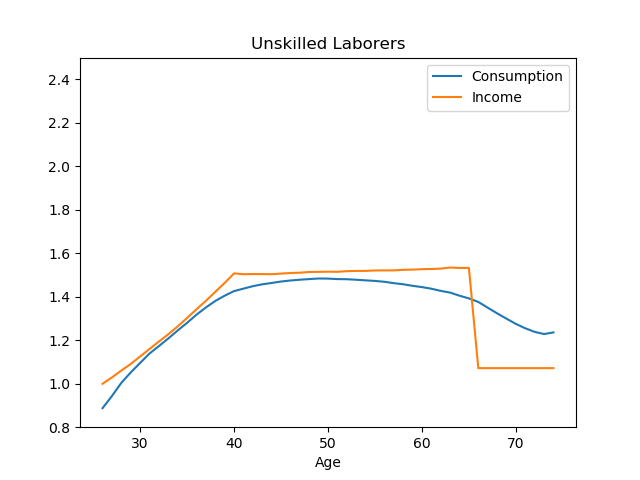
\includegraphics[width=4in]{Figures/Figure5a.png}}
\end{figure}

\newpage

For Operatives, labor income grows at 2.5$\%$ annually from the age 25 to 50, then 1$\%$ per year until retirement. \\
\begin{figure}[H] 
\centerline{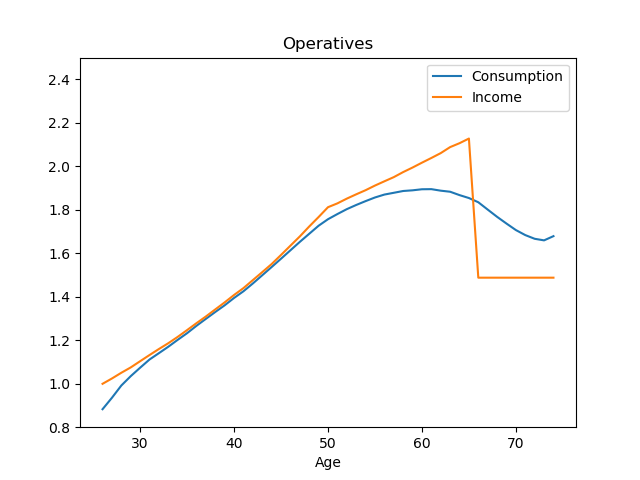
\includegraphics[width=4in]{Figures/Figure5b.png}}
\end{figure}

\medskip

For Managers, income grows at 3$\%$ from ages 25 to 55, and declines at 1$\%$ per year from 55 to 65.\\
\begin{figure}[H] 
\centerline{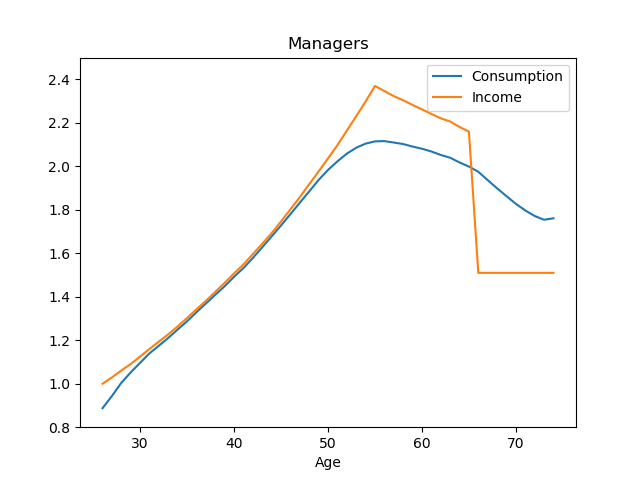
\includegraphics[width=4in]{Figures/Figure5c.png}}
\end{figure}

\section{Conclusion}

This paper argues that the buffer-stock version of the LC/PIH model is closer both to the behaviour of the typical household and to Friedman's original conception of the Permanent Income Hypothesis model. It can explain why consumption tracks income closely when aggregated by groups or in whole economies, but is often sharply different from income at the level of individual households. The model is consistent having higher MPC out of transitory income without imposing liquidity constraints. Further, it provides an explanation for why median household wealth/income ratios have remained roughly stable despite a sharp slowdown in expected income growth.



\newpage

\section{Appendix}
The following is a table showing the calibrated values of growth rates and etc. under different parameters.
\begin{table}[H]
	\label{table:1}
	\centerline{\scalebox{.7}{\begin{tabular}{lrrrrrrr}
\toprule
{} &  Growth rate of aggregate consumption &  Average growth rate of household permanent income &  Average growth rate of household consumption &  Aggregate personal saving rate &  Average MPC out of wealth &  Average net wealth &  Target net wealth \\
\midrule
Base Value         &                              0.020957 &                                           0.014807 &                                      0.014978 &                        0.006265 &                   0.315820 &            0.341770 &           0.313770 \\
g = .04            &                              0.040290 &                                           0.034225 &                                      0.034508 &                        0.009891 &                   0.414938 &            0.265945 &           0.246728 \\
depreciation = .10 &                              0.020821 &                                           0.014807 &                                      0.015143 &                        0.004310 &                   0.477366 &            0.230806 &           0.214614 \\
\bottomrule
\end{tabular}
}}
\end{table}

\newpage

\nocite{*}
\bibliographystyle{apacite}
\bibliography{\RefDir/Carroll1997}


\end{document}